\documentclass[a4paper,11pt,fleqn]{article}
%fleqn - opcja przesunięcia wzorów matematycnych
\usepackage{amssymb} %symbole matematyczne
\usepackage{amsmath} %musi być przed babelem z poowdu konfliktu komendy \lll

\usepackage[polish]{babel}
\usepackage[utf8]{inputenc}   % lub latin2
\usepackage[T1]{fontenc}
\usepackage{graphicx}
\usepackage{anysize}
\usepackage{enumerate}
\usepackage{times}
\usepackage{wrapfig}
\usepackage{framed}
 
%\marginsize{left}{right}{top}{bottom}
\marginsize{2cm}{2cm}{2cm}{2cm}
\sloppy
 
\begin{document}
\begin{wrapfigure}{R}{0.4 \textwidth}
\begin{framed}
\begin{center}

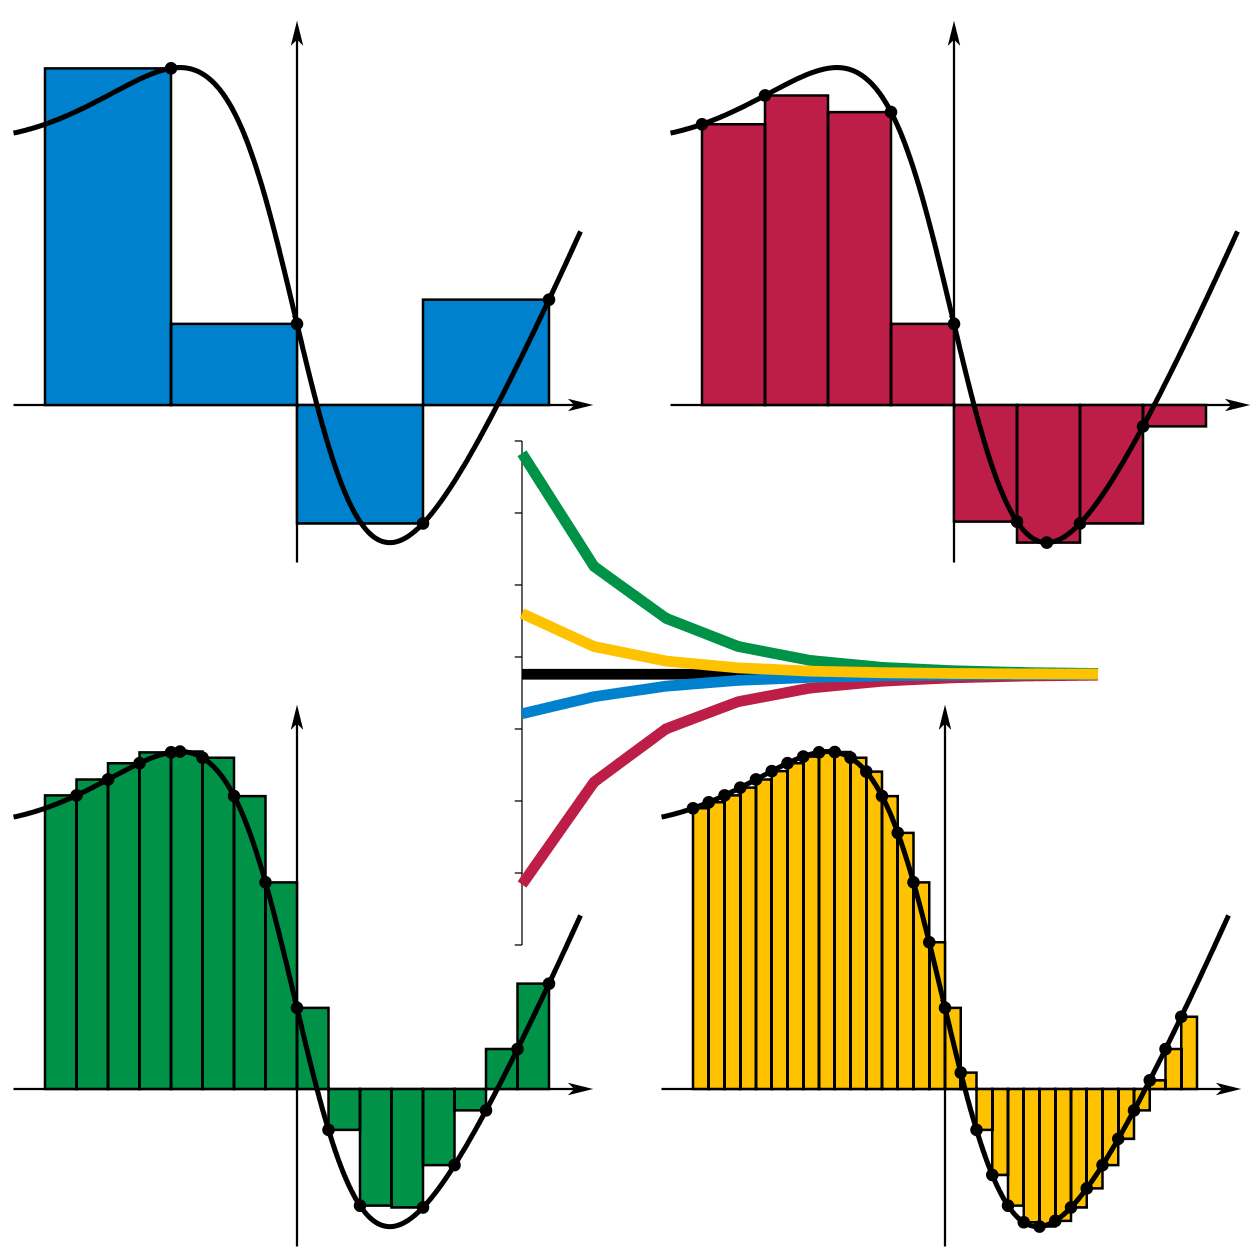
\includegraphics[width=\textwidth]{Plik_Riemann_sum_convergence.png}
\end{center}
\begin{flushleft}
\caption*{
\small
Przykład sum Riemanna przy wyborze punktu pośredniego w prawym końcu podprzedziału (niebieski), w wartości minimalnej (czerwony) i maksymalnej (zielony) funkcji w podprzedziale i lewego końca podprzedziału (żółty). Wartość wszystkich czterech przypadków zbliża się do 3,76 przy powiększaniu liczby podprzedziałów od 2 do 10 (w domyśle, również nieograniczenie).}
\end{flushleft}
\end{framed}
\end{wrapfigure}
\section*{Całka Riemmana}
 Niech dana będzie funkcja ograniczona 
 %\! - spacja ujemna
 $f\!\colon\![a,b]\to \mathbb {R} $.Sumą częściową (Riemanna) nazywa się liczbę
   \[R_{f,P(q_{1},\dots ,q_{n})}=\sum _{i=1}^{n}f(q_{i})\cdot \Delta p_{i}.\] %można też użyś $$ ale jest to niepolecane
Funkcję \(f\) nazywa się całkowalną w sensie Riemanna lub krótko R-całkowalną, jeśli dla dowolnego ciągu normalnego $(P^{k})$ podziałów przedziału $[ a , b ]$
istnieje (niezależna od wyboru punktów pośrednich) granica[b]
%
  \[ R_{f}=\lim _{k\to \infty }R_{f,P^{k}\left(q_{1}^{k},\dots ,q_{n_{k}}^{k}\right)}\]
%
nazywana wtedy całką Riemanna tej funkcji. Równoważnie: jeżeli istnieje taka liczba  ${\displaystyle R_{f},}$ że dla dowolnej liczby rzeczywistej $\varepsilon >0$ 
istnieje taka liczba rzeczywista $\delta >0$, że dla dowolnego podziału $P(q_{1},\dots ,q_{n})$ o średnicy ${\displaystyle \mathrm {diam} \;P(q_{1},\dots ,q_{n})<\delta ;}$ bądź też w języku rozdrobnień: że dla dowolnej liczby rzeczywistej $\varepsilon >0$ istnieje taki podział $S(t_{1},\dots ,t_{m})$ przedziału $[a,b]$, że dla każdego podziału
$P(q_{1},\dots ,q_{n})$  rozdrabniającego $S(t_{1},\dots ,t_{m})$ zachodzi
%
    \[\left|R_{f,P(q_{1},\dots ,q_{n})}-R_{f}\right|<\varepsilon \]
% 
Funkcję $f$nazywa się wtedy całkowalną w sensie Riemanna (R-całkowalną), a liczbę $R_f$ jej całką Riemanna.

\end{document}
